\chapter{Finalisierende Ausführungen}

In diesem letzten Kapitel werden Fazits bezüglich der eigenen Lernfortschritte in Bezug auf das Projekt als auch die Nutzung der Software thematisiert.

\section{Installations- und Administrationshandbuch}

In dieser Sektion werden das Installations- und Administrationshandbuch unterteilt.

\subsection{Installationshandbuch}

In diesem Installationshandbuch werden die einzelnen Schritte aufgeführt, die zur Installation der Software benötigt werden.

\begin{itemize}
    \item   \textit{Docker Desktop} mit WSL Command Line installieren (siehe hierzu Docker Desktop Installationsanleitung)
    \item   \textit{Node.js} installieren und das System neustarten
    \item   Eingabe in eine Kommandozeile: \textit{docker pull mongo}
    \item   In Docker Desktop nun das Image \textit{mongo} starten
\end{itemize}

\begin{figure}[!h]
    \centering
    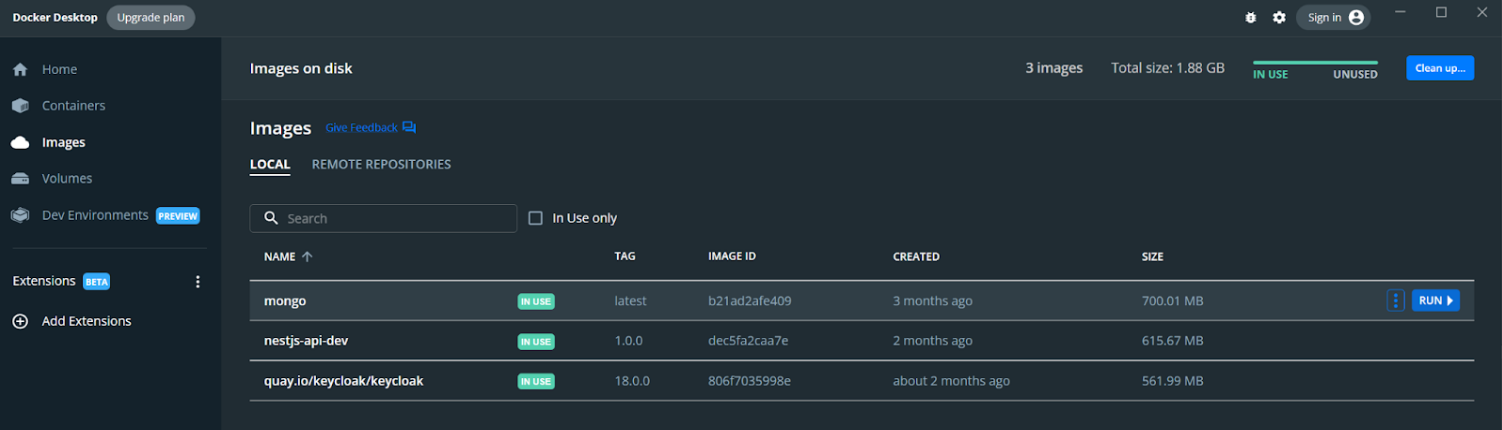
\includegraphics[width=0.8\textwidth]{6_1_Docker_MongoImage.png}
    \caption{Das Mongo Image highlighted in Docker Desktop}
    \label{fig:DockerMongoImage}
\end{figure}

\begin{itemize}
    \item   Bei der Konfiguration von Mongo in Docker Desktop muss unter dem Punkt \textit{Local Host} in \textit{Ports} folgendes eingegeben werden: \textit{27017}
    \item   Anschließend auf \textit{Run} klicken 
\end{itemize}

\begin{figure}[!h]
    \centering
    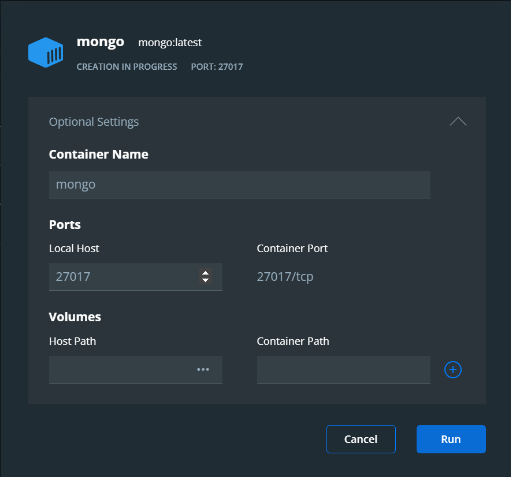
\includegraphics[width=0.8\textwidth]{6_1_Docker_MongoKonfig.png}
    \caption{So sollte die Konfiguration von Mongo aussehen nach dem letzten Schritt}
    \label{fig:DockerMongoKonfig}
\end{figure}

\begin{itemize}
    \item   Anschließend muss Keycloak gestartet werden, dazu muss in eine Kommandozeile folgendes eingegeben werden: \textit{docker run -p 8080:8080 -e KEYCLOAK\_ADMIN=admin -e KEYCLOAK\_ADMIN\_PASSWORD=admin quay.io/keycloak/keycloak:18.0.2 start-dev}
    \item   Nun in Docker Desktop unter dem Punkt \textit{Containers} den \textit{Keycloak} Container (erkennbar am Port 8080) und den \textit{mongo} Container starten
    \item   Im Browser kann dann die Route \textit{localhost:8080} aufgerufen werden und mit dem Nutzernamen \textit{admin} und Passwort \textit{admin} kann sich eingeloggt werden
    \item   Aus dem GitHub Repository dann die Datei \textit{realm-export.json} herunterladen
    \item   Unter \textit{Add Realm} eine Realm namens \textit{DeskPlanner} erstellen
    \item   Auf der linken Seite unter \textit{Import} die zuvor heruntergeladene Datei \textit{realm-export.json} auswählen
    \item   Unter \textit{existierenden Ressourcen Skip} auswählen und importieren 
\end{itemize}

\begin{figure}[!h]
    \centering
    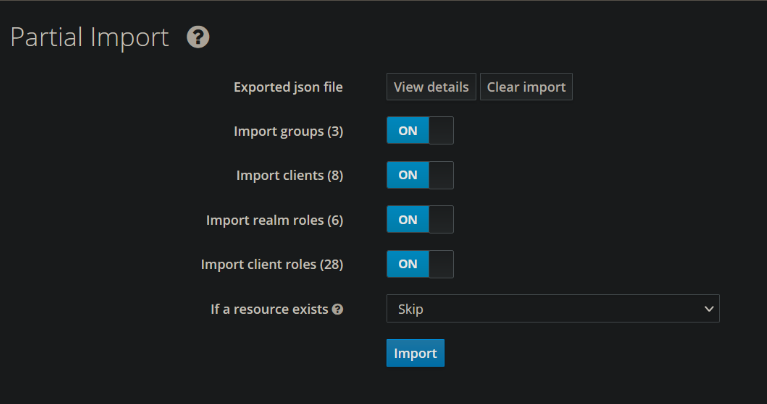
\includegraphics[width=0.8\textwidth]{6_1_Keycloak_Import.png}
    \caption{So sollte der Import aussehen}
    \label{fig:KeycloakImport}
\end{figure}

\begin{itemize}
    \item   Unter \textit{Users} einen neuen User anlegen mit \textit{Add User}
    \item   Anschließend die persönlichen Daten der Nutzer (\textit{Usernamen, Vor- und Nachnamen}) eingeben und speichern
    \item   Nun die User anklicken, dazu muss gegebenenfalls \textit{View all users} angeklickt werden
    \item   Hier kann unter \textit{Credentials} ein Passwort hinzugefügt werden
    \begin{description}
    \item[Wichtig:] Das Passwort muss als \textit{nicht-temporär} gespeichert werden
    \end{description}
    \item   In \textit{Role Mappings} im Dropdown \textit{Client Roles} muss \textit{keycloak-reactjs-demo} ausgewählt werden
    \item   Hier können die gewünschten Rollen \textit{(admin, mitarbeiter, ...)} gewählt werden
    \item   Anschließend muss in einem weiteren Konsolenfenster in den Ordner \textit{nestjs-desk-planner} mithilfe von \textit{cd} gewechselt werden
    \item   Nun folgenden Befehle eingeben und ausführen lassen: \textit{npm install}
    \item   Nach einem erfolgreichen ersten Befehl den nächsten: \textit{npm run start}
    \item   In der Umgebungsentwicklung in der Kommandozeile folgenden Befehl eingeben: \textit{cd ./react-user-app/}
    \item   Nun folgende Befehle eingeben und ausführen lassen: \textit{npm install --force} und anschließend \textit{npm start}
\end{itemize}

Nach erfolreichem Durchführen der Installationsanleitung sollte der DeskPlanner erfolgreich eingerichtet sein und kann anschließend benutzt werden.
Im Administrationshandbuch finden Sie weitere Informationen zur Konfiguration und zur Benutzung des RaumEditor für den Administrator.
\subsection{Administrationshandbuch}

\begin{figure}[!h]
    \centering
    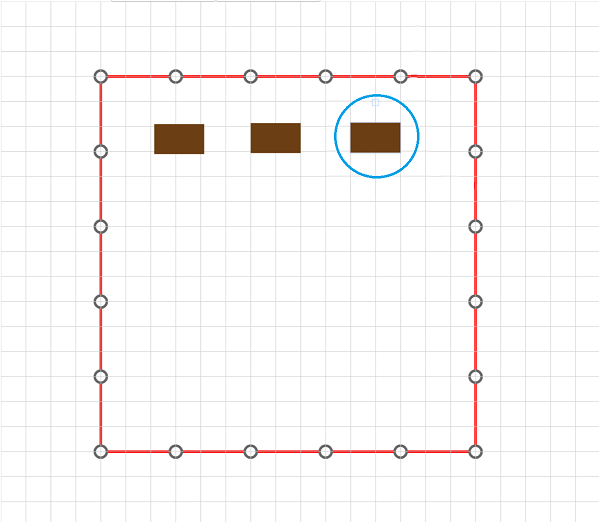
\includegraphics[width=0.8\textwidth]{RaumEditor.png}
    \caption{Layout Designer - Administrator}
    \label{fig:LayoutDesigner}
\end{figure}

Als Administrator des IT-Systems ist seine hauptsächliche Aufgabe die Verwaltung von Gebäuden, Stockwerken und Räumen im Layout Designer.
In diesem kann der Administrator einen zuvor definierten Bereich anhand der weißen Kugel-Komponenten editieren, um das richtige Raumlayout mit den eingezeichneten roten Linien zu erstellen.
Außerdem ist es möglich, mit einem Doppel-Klick eine braune Tisch-Komponente (in der Abbildung blau gekennzeichnet) zu erstellen und diesen beliebig im Raum zu verteilen.
Diese Tische können ebenfalls mit einem Rechts-Klick gelöscht werden.
Für den Administrator befindet sich ein kleines Tutorial im Layout Designer, welcher die Funktionsweise des Layout Designers erklärt.
Hier kann der Administrator den Raum erstellen und angeben, wo dieser sich befindet, um den Arbeitnehmern im Buchen Bereich vorgefertigte Räume zu geben, welche dann gesucht und gebucht werden können.

\pagebreak

\section{Reflektion: Aufteilung des Teams}

\begin{figure}[!h]
    \centering
    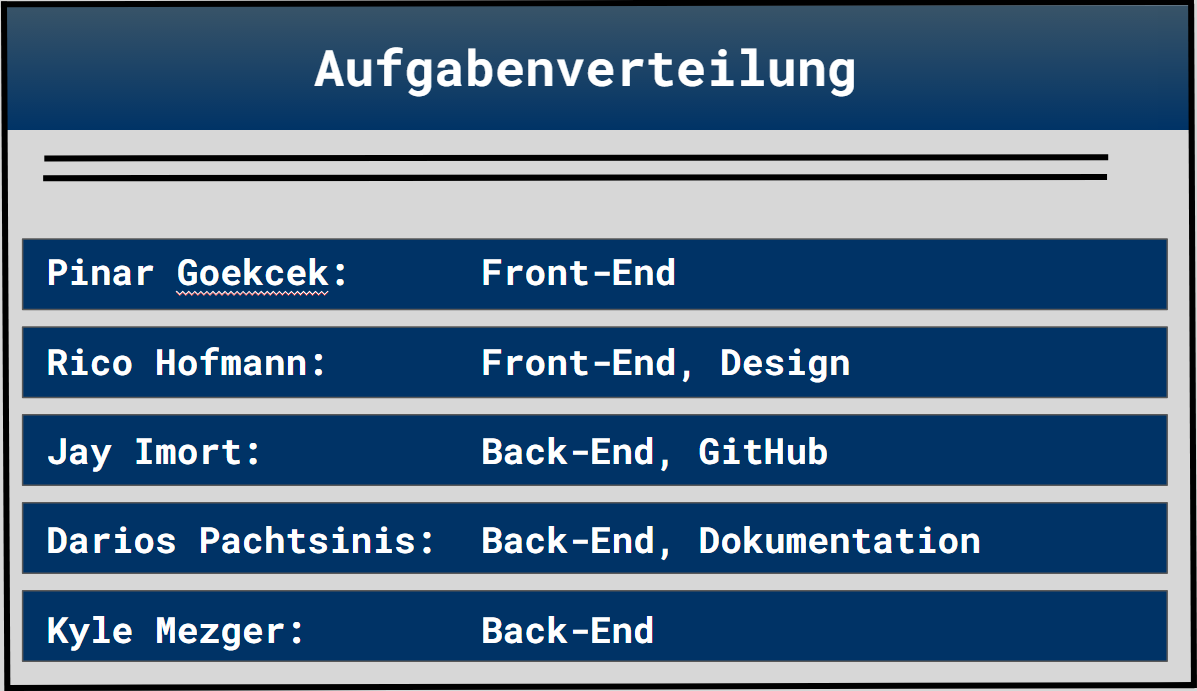
\includegraphics[width=0.8\textwidth]{Aufgabenverteilung.png}
    \caption{Aufgabenverteilung - Erste Präsentation}
    \label{fig:Aufgabenverteilung}
\end{figure}

In der Abbildung zu erkennen, ist die erste Aufgabenverteilung im Vorfeld des Projekts.
Die Aufteilung fand grob in Front-End und Back-End statt, mit kleinen Aufgabenspezifikationen wie Design, GitHub und Dokumentation.
Diese Aufteilung beruht auf vergangene Projekte im Rahmen des Studiums.

Nachdem das Projekt begonnen wurde, wurde die Aufteilung weiter ausgebaut.
Im Vorfeld war klar, dass Rico Hofmann als Front-End Entwickler fungiert, da seine vergangenen Aufgaben rund um das Thema Design vorangegangene Projekte prägten.
Rico Hofmann ist somit der Lead Designer des Teams, denn er baute das Grundgerüst für die Design-Aufgaben, welche später von Darios Pachtsinis und Pinar Gökcek erweitert und vollendet wurden.
Des Weiteren ist Rico der Experte für Material UI und führte außerdem auch das Protokoll für Teambesprechungen mit unserem Betreuer.

Kyle Mezger ist einer der Back-End Entwickler, welcher sich zur Aufgabe machte, die REST API zu erstellen und auszubauen und den Login via Keycloak zu verwalten.
Er hatte sich allerdings auch um die Kommunikation mit dem Betreuer als auch für die wöchentliche Aufgabenverteilung innerhalb der Gruppe via Issues in GitHub gekümmert.

Jay Imort hingegen ist der andere Back-End Entwickler, welcher seinen Fokus hauptsächlich auf Nest.js, Routing legt.
Des Weiteren beschäftigte er sich mit dem Layout Designer, in welchem der Benutzer einen Raumlayout erstellen, bearbeiten und in die Datenbank laden kann.

Die Aufgaben im Back-End Bereich wurden meist vermischt und deswegen teilten sich Kyle Mezger und Jay Imort die Aufgaben gerecht und deren Fachwissen entsprechend auf.

Darios Pachtsinis wurde ursprünglich dem Back-End Team zugeteilt, allerdings hatte das Team mehr Designer gebraucht, weswegen sein Aufgabenfeld doch zum Front-End zugeteilt worden ist.
Er hatte Aufgaben erledigt wie das Finalisieren von Design Entscheidungen, hauptsächlich rund um den Buchungen Bereich (Booking, etc.).

Pinar Gökcek ist ebenfalls im Front-End zuständig gewesen und hatte Design Entscheidungen von Rico Hofmann finalisiert.
Außerdem erledigte sie Aufgaben speziell im Nachrichten Bereich (Messages, etc.), wie das Empfangen von Nachrichten, als auch dessen Verknüpfung mit der Datenbank.

Zu guter Letzt jedoch war das Team kein Zusammenschluss von 5 Einzelpersonen mit Fachwissen in besonderen Bereich, sondern das Team unterstützte sich gegenseitig, sodass jeder auch außerhalb des zuvor genannten Aufgabenbereichs Aufgaben erledigen konnte.
Dies bedeutet, dass das Team sich immer helfen konnte, sich gegenseitig motiviert hat und auf die Erledigung der Aufgaben anderer achtete und tatkräftig unterstützt hatte.
Die Aufgabenverteilung ist somit grob und soll verdeutlichen, dass die Übergänge zu anderen Aufgabenbereichen und Teammitgliedern vermischen.

\section{Reflektion: Projektmanagement}

Als Projektmanagement wurde eine Mischung aus Kanban und Scrum, auch Scrumban, genutzt.
Wie im Voraus erwartet, hatte uns das Kanban Board eine große Hilfe geleistet beim Überblicken der Projektaufgaben.
Das Kanban Board wurde mit einem von GitHub bereitgestellten Issue-System verbunden, welches wir nutzten, um größere Aufgabenteile zu unterteilen und diese einem Mitglied zuzuweisen.

Mithilfe der wöchentlichen Meetings konnten wir uns gut koordiniert auf die Aufgaben des Boards konzentrieren und diese auch größtenteils bewältigen.
Wir setzten unser wöchentliches Meeting auf den Dienstag, um den Montag mit unserem Betreuer zu nutzen.
Die Vorstellung unseres jeweiligen Standes, gab uns mindestens eine weitere Expertenmeinung, welche wir für unser Gruppenmeeting nutzten.
Um diese Expertenmeinung bestmöglich zu nutzen, haben wir ebenfalls für jedes Treffen ein Protokoll geführt, welches wir direkt in unsere Aufgabenbesprechungen untergebracht hatten.


